\section{Shor's Algorithm}
\subsection{Modulo Operations and Relevant Mathematical Background}
\begin{definition}
    A prime number $p \in \Z^+$ is a number that has no divisors other than $1$ and $p$.
\end{definition}
\begin{theorem}
    The \uimpt{Fundamental Theorem of Arithmetic} states that for all positive integers $x$, $x$ can be factored into a product of primes. Moreover, the factorization is unique (up to re-ordering).
\end{theorem}
Given a positive interger $N$, let $x, y \in \Z$, we write
$$x \bmod N$$
to mean the unique element $x' \in \{0, \dots, N-1\}$ such that $N$ divides $(x - x')$. \\
We write
$$x \equiv y \pmod N$$
to mean that $x \bmod N = y \bmod N$.
\begin{definition}
    Given $a, b \in \Z$, not both zero, the \uimpt{greatest common divisor} of $a$ and $b$ is the largest $d \in \Z^+$ such that $d$ divides $a$ and $d$ divides $b$. We write:
    $$\gcd(a, b) = d$$
\end{definition}
\begin{definition}
    $a, b$ are co-prime if $\gcd(a, b) = 1$.
\end{definition}
\begin{definition}
    Let $a, N \in \Z^+$, if $\gcd(a, N) = 1$, and $\exists r \in \Z^+$ where $a^r \equiv 1 \pmod N$, the least such $r$ is called \uimpt{the order of $a$ modulo $N$}, denoted as
    $$\ord{N}{a}$$
\end{definition}
We only consider the case where $N = pq$, for $p, q$ being distinct primes. \\
We describe the algorithm in three steps:
\begin{quote}
    1. Choose $a$ uniformly at random from the set $\{1, \dots, N-1\}$, compute $d := \gcd(a, N)$. If $d > 1$, output $d$. Otherwise, we know $a$ and $N$ are co-prime. \\
    2. Compute $r := \ord{N}{a}$ \impt{on a quantum computer}. If $r$ is odd, output ``do not know'', otherwise, continue to Step 3. \\
    3. Compute $d' := \gcd(a^{\frac{r}{2}} - 1 \bmod N, N)$. If $d' > 1$, output $d'$. Otherwise, output ``do not know'' and the algorithm fails for this instance.
\end{quote}
This algorithm will always output the correct answer if it does not output ``do not know''.
\begin{theorem}
    Suppose $a$ is chosen u.a.r from $\{a' \in \{1, \dots, N-1\} \mid \gcd(a', N) = 1\}$, then
    $$\Prob{2 | r := \ord{N}{a} \land a^{\frac{r}{2}} \ne -1 \bmod N} \ge \frac{1}{2}$$
\end{theorem}
\begin{theorem}
    $$\Prob{\text{``do not know''}} \le \frac{1}{2}$$
\end{theorem}

\subsection{Quantum Fourier Transform}
\begin{definition}
    Let $M \in \Z^+$, the \uimpt{quantum fourier transform} on $\C^M$ is the unitary defined by
    $$\text{QFT}_M \ket{j} = \frac{1}{\sqrt{M}} \Sum{k = 0}{M -1} \omega_M^{k \cdot j} \ket{k}$$
    for $j \in \{0, 1, \dots, M-1\}$ and
    $$\omega_M = \exp(\imag \frac{2\pi}{M})$$
\end{definition}
The quantum circuit that computes $r := \ord{N}{a}$ is the following:
\begin{center}
    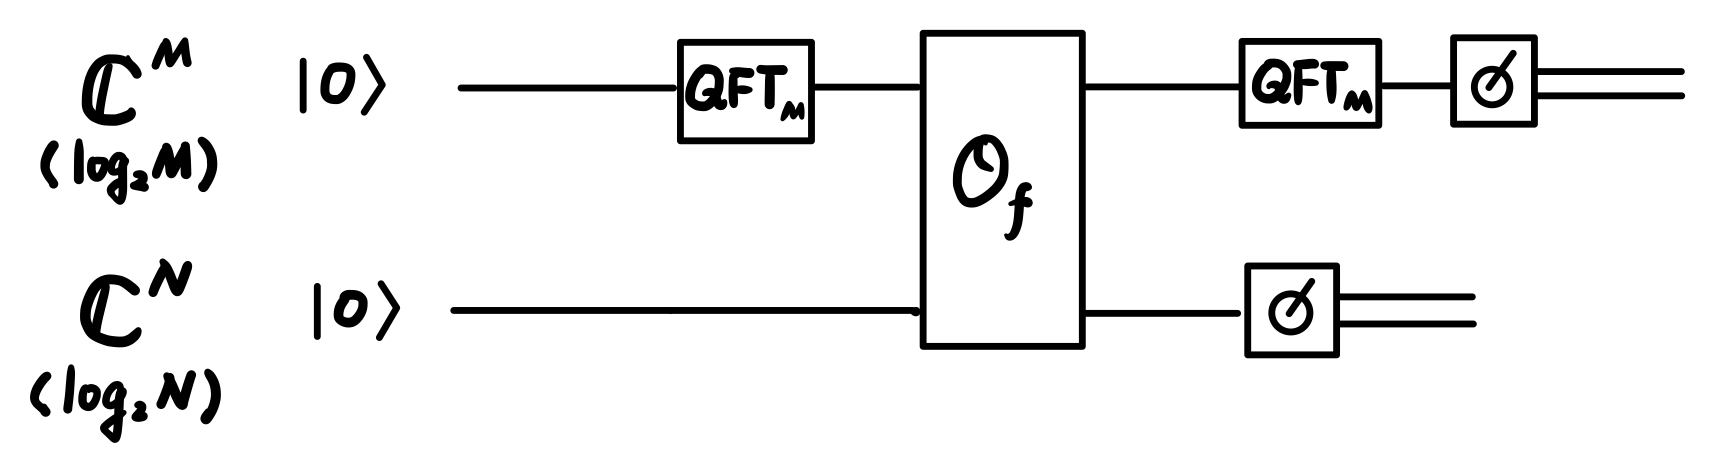
\includegraphics[scale = 0.2]{8/qft.png}
\end{center}
where we have:
\begin{align*}
    f: \{0, 1, 2, \dots, M-1\} &\to \{0, 1, \dots, N-1\} \\
    x &\mapsto a^x \bmod N
\end{align*}
We take $M > N^2$ and assume $M = \lambda r$ for some $\lambda \in \Z^+$. \\
After we measure the second qubit and obtain some $f(k)$ for $k \in \{0, 1, \dots, r - 1\}$, the first qubit collapes to:
$$\frac{1}{\sqrt{\lambda}} \Sum{l = 0}{\lambda - 1} \ket{k + l r}$$
where $l \in \{0, 1, \dots, \lambda - 1\}$. \\
After applying $\QFT$ on the first qubit, measurement on the first qubit, gives $n\lambda$ where $n$ is chosen u.a.r from $\{0, 1, \dots, r - 1\}$. \\
We extract $r$ by the following:
\begin{quote}
    1. Divide $n\lambda$ by $M$ to get $f := \frac{n}{r}$. \\
    2. Express $f$ in its simplest terms and read off the denominator, call $r'$. \\
    3. Verify if $a^{r'} \equiv 1 \bmod N$, if yes give $r'$, if not give ``fail''.
\end{quote}
There are two cases, if $n$ is co-prime to $r$, then $r' = r$, which occurs with probability $\ge \gamma$; if $n$ is not co-prime to $r$, $r$ is a multiple of $r'$. Then doing $\order{\frac{1}{\gamma}}$ repeats of the algorithm ensures with almost certainty that we land in the first case and obtain $r$. \\
The complexity of each repeat is $\order{\log^3 N}$ and $\frac{1}{\gamma} \sim \log(\log N)$. \\
The QFT circuit is implemented in the following way:
\begin{center}
    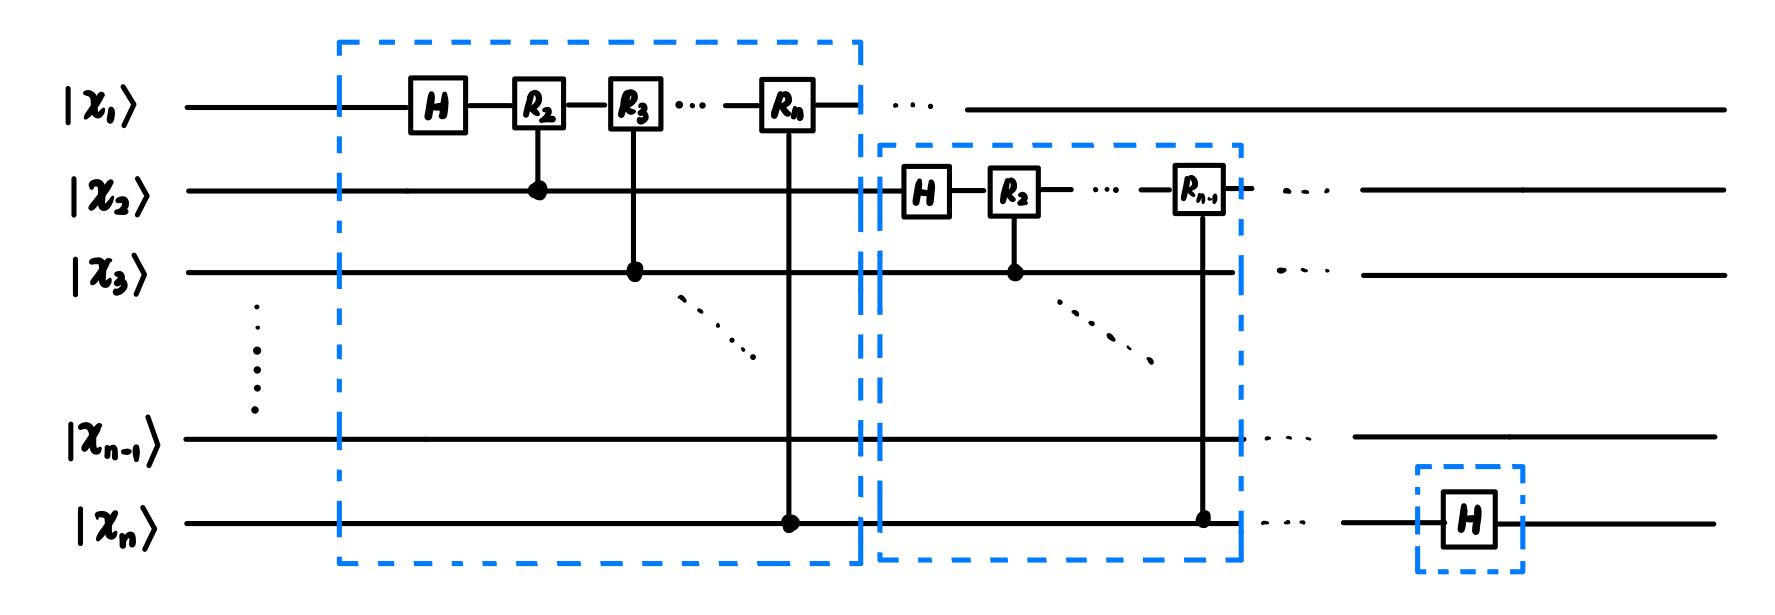
\includegraphics[scale = 0.2]{8/qft_circuit.png}
\end{center}
where
$$R_k = \begin{pmatrix}
    1 & 0 \\
    0 & e^{\imag \frac{2\pi}{2^k}}
\end{pmatrix}$$
This circuit is realized using $\order{n^2} \sim \order{\log^2 N}$ quantum gates.

\newpage